\documentclass[12pt,letterpaper,noanswers]{exam}
\usepackage[usenames,dvipsnames,svgnames,table]{xcolor}
\usepackage[margin=0.9in]{geometry}
\renewcommand{\familydefault}{\sfdefault}
\usepackage{multicol}
\pagestyle{head}
\header{AM 111 Class 19}{}{Initial value problems: differential equations, p.\thepage}
\runningheadrule
\headrule
\usepackage{siunitx}
\usepackage{graphicx} % more modern
\usepackage{amsmath} 
\usepackage{amssymb} 
\usepackage{hyperref}
\usepackage{tcolorbox}
\usepackage{enumitem}
\def\mbf{\mathbf}
\newcommand{\vc}[1]{\boldsymbol{#1}}
\def\dsst{\displaystyle}
\DeclareMathOperator*{\argmin}{arg\,min} % thin space, limits underneath in displays
\usepackage[numbered,autolinebreaks,useliterate]{mcode}

\begin{document}
 \pdfpageheight 11in 
  \pdfpagewidth 8.5in

\noindent 

\section*{Preliminaries}

\begin{itemize}
\itemsep0pt
\item Your problem set, project proposal, and individual project timeline are due tomorrow.
\item Your third self-reflection is due before class on Tuesday.  It is available on Gradescope now.
\item Your out of class assignment next week will be project work.
\item There is a skill check in the next class.
\end{itemize}


\noindent\textbf{Big picture}

Today: 

\vspace{0.2cm}
\hrule
\vspace{0.2cm}

\noindent \textbf{Skill check practice}
\begin{questions}
\item The midpoint method is given by $y_{k+1} = y_k + h\psi(t_k,y_k,h)$ where $\psi(t_k,y_k,h) = f(t_k+h/2,y_k+hf(t_k,y_k)/2)$.

Use Taylor expansion to first order to write $f(t_k+h/2,y_k+hf(t_k,y_k)/2)$ in terms of $f(t_k, y_k)$,$\dfrac{\partial f}{\partial t}(t_k,y_k)$, $\dfrac{\partial f}{\partial y}(t_k,y_k)$, and $\mathcal{O}(h^2)$.

\item The skill from the Class 17 handout (Skill Check C18).
\end{questions}


\vspace{0.2cm}
\hrule
\vspace{0.2cm}

\noindent \textbf{Skill check solution}
\begin{questions}
\item

Taylor expanding about $f(t_k, y_k)$, the displacement in time is $\Delta t = h/2$ and the displacement in $y$ is $\Delta y = hf(t_k,y_k)/2$.

In general, $f(t+\Delta t, y+\Delta y) = f(t,y) + \Delta t \dfrac{\partial f}{\partial t}(t,y) +  \Delta y \dfrac{\partial f}{\partial y}(t,y) + \text{higher order terms}$


Applying this:

$f(t_k+h/2,y_k+hf(t_k,y_k)/2) = f(t_k,y_k) + \dfrac{h}{2} \dfrac{\partial f}{\partial t}(t_k,y_k) + \dfrac{h}{2}f(t_k,y_k) \dfrac{\partial f}{\partial y}(t_k,y_k) + \mathcal{O}(h^2)$

\item See the past handout.
\end{questions}
\vspace{0.2cm}
\hrule
\vspace{0.2cm}

\noindent \textbf{Teams}
\begin{multicols}{3}
1. Mina, Basil, Johan

2. Nini, Brian, Eli

3. Nicolas, Aidan, Julia K

4. Mack, Benjamin, Robert

5. Alex, RJ, Jessica

6. Caitlin, Nina, Daniyal

7. Cameron, Dani, Emma

8. Eletria, Julia M, Tom

9. Ray, Ivonne, Shang

10.  Sophie, Eric, Alex

11. Jack, Esmé, Zachary

12. Kevin, Kevin, Marissa

\end{multicols}


\section*{Ordinary differential equations}
\subsection*{Explicit methods (see Greenbaum and Chartier \S 11.2}
\begin{tcolorbox}
Let $y_k$ denote the approximation to $y(t_k)$ produced by our numerical method.
\begin{itemize}
\itemsep0pt
    \item An \textbf{explicit} one-step method can be written in the form $y_{k+1} = y_k + h \psi(t_k,y_k,h)$ where $\psi(t_k,y_k,h)$ is an estimate of the effective slope of $y(t)$ over the interval $[t_k,t_{k+1}]$.
    \item Euler's method is one such method: $\psi(t_k,y_k,h) = f(t_k,y_k)$, the estimated slope at the beginning of the interval.
    \item The \textbf{midpoint method} is another such method.  Use a slope estimate at the middle of the interval for $\psi$.  Compute half a step using Euler's method: $y_{k+1/2} = y_k + h/2f(t_k,y_k)$.  $\psi(t_k,y_k,h) = f(t_{k+1/2},y_{k+1/2}) = f\left(t_k + h/2, y_k+\frac{h}{2}f(t_k,y_k)\right)$
    \item Heun's method, or \textbf{improved Euler} is another such method.  Use an average of the slope at $t_k$ and the Euler estimate of the slope at $t_{k+1}$: $\psi(t_k,y_k,h) = f(t_k,y_k)/2 + f(t_k + h,y_k+hf(t_k,y_k))/2$
\end{itemize}
\end{tcolorbox}

\begin{enumerate}[resume=classQ]
    \item The plot below is showing the global error of four different methods as a function of step size.  The error was generated by comparing the approximate solution via the method to a known exact solution (for a particular differential equation).
    \begin{parts}
    \item How can you tell the order of the methods in the plot of error below?
    \item What is the order of each method?  
    \item For the methods where the error reaches a minimum, why is that happening?
    \end{parts}
    
      
\end{enumerate}
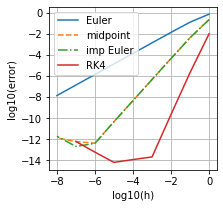
\includegraphics[]{img/C18error.png}
\begin{tcolorbox}
Explicit \textbf{Runge-Kutta} methods use intermediate estimates of $y$ in the interval $[t_k,t_{k+1}]$ in order to create $\psi(t_k,y_k,h)$.  
\begin{itemize}
\itemsep0pt
    \item Improved Euler is a second order Runge-Kutta method.
    \item The \textbf{classical fourth-order Runge-Kutta method} (RK4) is given by 
    
    $q_1 = f(t_k,y_k)$, 
    
    $q_2 = f(t_k+h/2,y_k+\frac{h}{2}q_1)$
    
    $q_3 = f(t_k + h/2,y_k + \frac{h}{2}q_2)$
    
    $q_4 = f(t_k+h, h_k + hq_3)$
    
    $\psi(t_k,y_k,h) = \frac{1}{6}(q_1+2q_2+2q_3+q_4)$
\end{itemize}
\end{tcolorbox}
\begin{enumerate}[resume=classQ]
\item When $f(t,y)$ depends only on $t$, we have $\dfrac{dy}{dt} = f(t)$.  Find a simplification of Euler's method for this case.  (What method is this?)
\vspace{1in}
\end{enumerate}

\subsection*{Implicit methods}
\begin{tcolorbox}
\begin{itemize}
\itemsep0pt
    \item The \textbf{backward Euler} method is $y_{k+1} = y_k + hf(t_{k+1},y_{k+1})$.  This is an \textbf{implicit} equation for $y_{k+1}$: $y_{k+1}$ is an unknown and appears on both sides of the equation.
    \item Implicit Runge-Kutta (IRK) methods also exist (and the weights are related to Gaussian quadrature, see Greenbaum and Chartier \S 11.4.3).
\end{itemize}
\end{tcolorbox}

\begin{enumerate}[resume=classQ]
\item Let $\dfrac{dx}{dt} = -x^3/3 + x + \alpha$.  Set $\alpha = 2/3, x(0) = 2$.  Set up an implicit equation for finding $x_1$ using the backwards Euler method ($x_0 = x(0) = 2$).
\vspace{1in}
\item (Greenbaum and Chartier \S 11.6 Q 16) A simple model for a muscle controlling a heart valve is given by \[\displaystyle\begin{array}{l} dx/dt = -x^3/3 + x + \alpha \\
d\alpha/dt= -\epsilon x \end{array}\]
where $x$ is the position of the muscle and $\alpha$ is the concentration of a chemical stimulus.

Let $\epsilon = 0.01, x(0) = 2, \alpha(0) = 2/3$.  Set up a pair of implicit equations for $x_1, \alpha_1$ using the backwards Euler method.  

Note: $x_{k+1} = x_k + hf(t_{k+1},x_{k+1},\alpha_{k+1})$, $\alpha_{k+1} = \alpha_k + hf(t_{k+1},x_{k+1},\alpha_{k+1})$ 
\vspace{1in}
\end{enumerate}
\begin{tcolorbox}
\begin{itemize}\itemsep0pt
        \item To use backward Euler requires solving a nonlinear equation with one unknown at each step.  That means it requires the use of a root finding method.
    \item When using an implicit method, it is typical to use an explicit method to make a guess of the value of $y_{k+1}$ (a \textbf{predictor step}), and then take a \textbf{corrector step} using the implicit method.
\end{itemize}
\end{tcolorbox}
\subsection*{Stiff equations (Greenbaum and Chartier \S 11.4)}

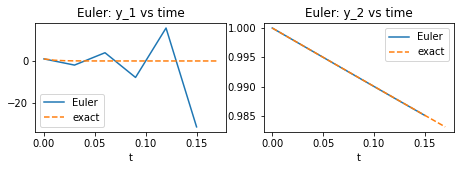
\includegraphics{img/C19stiff.png}
\begin{enumerate}[resume=classQ]
\item For the system
\begin{align*}
    y_1' &=-100y_1+y_2 \\
    y_2' &= -0.1 y_2
\end{align*}
the exact solution is given by $y_2(t) = y_2(0)e^{-0.1t}$ and $y_1(t) = e^{-100t}(y_1(0) - 10y_2(0)/999)+e^{-0.1t}10y_2(0)/999$.
\begin{parts}
\item Let $y_1(0) = y_2(0) = 1$.  Based on the exact solution, how should $y_1$ and $y_2$ evolve with time?  Will their values increase or decrease?
\vspace{1cm}
\item In the plot above, using Euler's method with $h = 0.03$, how do the approximated solutions evolve with time?
\vspace{1cm}
\end{parts}
\end{enumerate}

\begin{tcolorbox}
When equations have components evolving on very different time scales they are called \textbf{stiff} equations.
\begin{itemize}
\itemsep0pt
    \item For the example of stiff equations above, Euler's method fails for step sizes above $h<0.02$: it fails by generating growth and oscillation instead of expontial decay.
    \item This type of failure is called \textbf{instability}.
\end{itemize}
\end{tcolorbox}
\begin{tcolorbox}
To assess stability of the method, use the test equation $dy/dt = \lambda y$, with $\lambda \in \mathbb{C}$.
\begin{itemize}
\itemsep0pt
\item For $\lambda = a + ib$ with $a,b\in\mathbb{R}$, the exact solution to the test equation is $y(t) = y_0e^{\lambda t} = y_0e^{at}e^{ibt} = y_0e^{at}(\cos bt + i \sin bt)$.  It decays to $0$ for $a<0$, which corresponds to the left half of the complex plane.
    \item Apply a numerical method, with step size $h$, to the test equation.  Find the set of $h\lambda \in \mathbb{C}$ such that $y_k\rightarrow 0$ as $k\rightarrow\infty$.
    \item This is the region of \textbf{absolute stability} of the method.
    \item A method is called \textbf{A-stable} when the entire left half plane is in its region of absolute stability.
\end{itemize}
\end{tcolorbox}
\begin{enumerate}[resume=classQ]
    \item You applied the forward Euler method to $dy/dt = cy$ in the last class.  For this method, with $dy/dt = \lambda y$, $y_{k+1} = y_0(1+h\lambda)^{k+1}$.  
    \begin{parts}
    \item Find a mathematical expression for the region of absolute stability (the set of $h\lambda \in \mathbb{C}$ such that $y_k\rightarrow 0$ as $k\rightarrow \infty$).
    \vspace{1in}
\item To help you plot this region in the complex plane, write $h\lambda = x + iy$, and find the set of points $(x,y)$ that satisfy the condition.
\vspace{1in}
    \end{parts}


    \item Apply the backwards Euler method to the test equation.
    \begin{parts}
    \item First find an expression for $y_{k+1}$ in terms of $y_k$.  Then find an expression for $y_{k+1}$ in terms of $h,\lambda,k, y_0$.
    \vspace{1in}
    \item Find a mathematical expression for the region of absolute stability.
    \vspace{1.5cm}
    \item To help you think about this region in the complex plane, again write $h\lambda = x + iy$.  Argue that for $x<0$ the condition you found will always be true.
    \vspace{1in}
    \end{parts}
    The backwards Euler method is A-stable.
\end{enumerate}
%\subsection*{Implementation considerations (Greenbaum and Chartier \S 11.2.8)}
\end{document}